\subsection*{Aufgabe 3}

a) Folgende Anweisungen wurden parallel ausgeführt: 

\begin{enumerate} 
  \item x++
  \item y++
  \item y += 2
  \item y = x + 2
  \item x = y + 3
\end{enumerate}

Ich gehe bei der Bearbeitung der Aufgabe davon aus, dass x und y mit 0 initialisiert wurden. 
Die letzen beiden Befehle  sind die einzigen die x und y in beziehung setzten. Die anderen Befehle erhöhen nur den wert der jeweiligen Variablen. Außerdem können sich die Befehle gegnseiteig beim schriebn überlagern. Somit sind 2 Situationen denkbar:
\begin{itemize}
  \item Befehl 4,5 am Anfang
  \item Befehl 4,5 irgendwo in der Mitte oder ganz am Ende 
\end{itemize}

Im ertsehn fall verändern die Variablen sich nicht und somit sind folgende paare Möglich:
\begin{itemize}

	\item[] y = 2, x = 3
	\item[] y = 2, x = 4
	\item[]

	\item[] y = 3, x = 3
	\item[] y = 5, x = 3
	\item[]

	\item[] y = 3, x = 4
	\item[] y = 5, x = 4
\end{itemize}


Im zweiten fall könn zusätzlich noch folgende Konstalationen hinzukommen
\begin{itemize}
	\item[] y = 2, x = 5
	\item[] y = 2, x = 6
	
	\item[] y = 3, x = 6
	\item[] y = 5, x = 8

	\item[] y = 3, x = 7
	\item[] y = 5, x = 9

	\item[] y = 5, x = 3
	\item[] y = 6, x = 4

	\item[] y = 6, x = 3
	\item[] y = 8, x = 3

	\item[] y = 7, x = 4
	\item[] y = 9, x = 4
\end{itemize}

\newpage

b)

Nach dem Einfügen der Angegenen Daten sieht der Baum wie folgt aus.

\begin{figure}[ht]
	\centering
  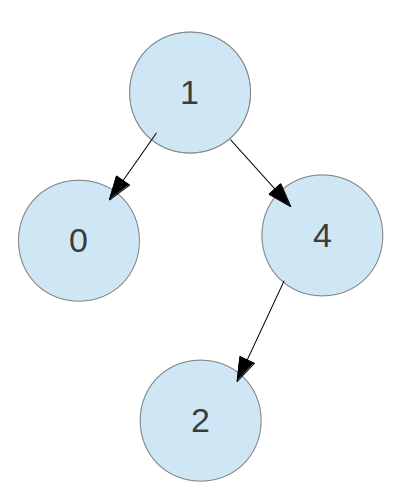
\includegraphics[width=0.33\textwidth]{baum}
	\caption{eingeügte Daten}
	\label{fig1}
\end{figure}

Beim Parallelen Einfügen und Löschen können eine Reihe von Fehlern entstehen. Unter anderem kann der Knoten mit dem Wert 3 so eingefügt werden, dass er direkt auf die Wurzel des Baumes zeigt.

\begin{figure}[ht]
	\centering
  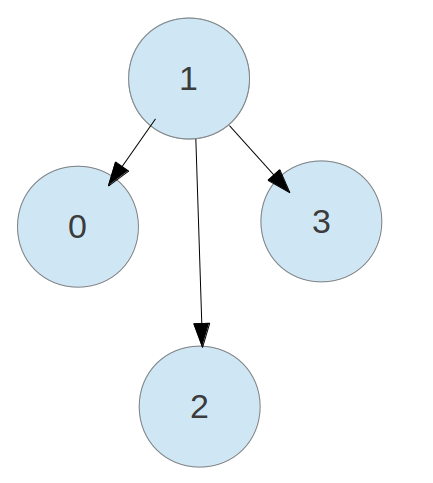
\includegraphics[width=0.33\textwidth]{problem}
	\caption{Fehler beim Einfügen}
	\label{fig1}
\end{figure}
